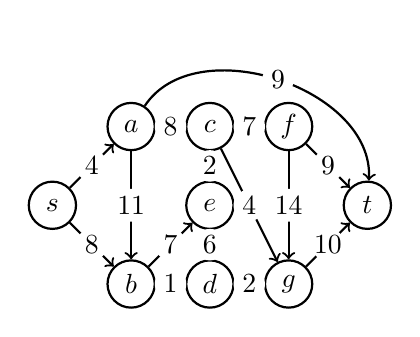
\begin{tikzpicture}[->, thick, main/.style = {circle,draw, inner sep = 0pt, minimum size = 0.6cm}, edge/.style = {circle, midway, fill=white, inner sep=0pt, minimum size=0.4cm}, scale = 0.5]    \node[main] (s) at (0, 0) {$s$};
    \node[main] (a) at (2, 2) {$a$};
    \node[main] (b) at (2, -2) {$b$};
    \node[main] (c) at (4, 2) {$c$};
    \node[main] (d) at (4, -2) {$d$};
    \node[main] (e) at (4, 0) {$e$};
    \node[main] (f) at (6, 2) {$f$};
    \node[main] (g) at (6, -2) {$g$};
    \node[main] (t) at (8, 0) {$t$};
    \path
        (s) edge[bend right = 0] node[edge] {4} (a)
        (s) edge[bend right = 0] node[edge] {8} (b)
        (a) edge[bend right = 0] node[edge] {11} (b)
        (a) edge[bend right = 0] node[edge] {8} (c)
        (c) edge[bend right = 0] node[edge] {7} (f)
        (c) edge[bend right = 0] node[edge] {2} (e)
        (e) edge[bend right = 0] node[edge] {6} (d)
        (b) edge[bend right = 0] node[edge] {1} (d)
        (b) edge[bend right = 0] node[edge] {7} (e)
        (c) edge[bend right = 0] node[edge] {4} (g)
        (d) edge[bend right = 0] node[edge] {2} (g)
        (f) edge[bend right = 0] node[edge] {14} (g)
        (f) edge[bend right = 0] node[edge] {9} (t)
        (g) edge[bend right = 0] node[edge] {10} (t)
        (a) edge[bend right = -75.0] node[edge] {9} (t);
\end{tikzpicture}